% !TeX root = ./main.tex
\documentclass[main]{subfiles}
\begin{document}
\chapter{Длина кривой}
\begin{definition}[Длина кривой]
    $\vf: [a,b] \to \R^3$, $a = t_0 < t_1 < ... < t_n = b$, $\Delta_i t = t_i - t_{i-1}$.
    \[L \coloneqq \lim_{\max \Delta_i t \to 0} \sum_{i=1}^n |\vf(t_i) - \vf(t_{i-1})|\]
\end{definition}

\begin{definition}[Спрямляемая кривая]
    Прямая называется спрямляемой, если существует её длина.
\end{definition}
\begin{example}
    $y = \sin 1/x$  на $(0, 1]$ не спрямляемая.
    \begin{center}
        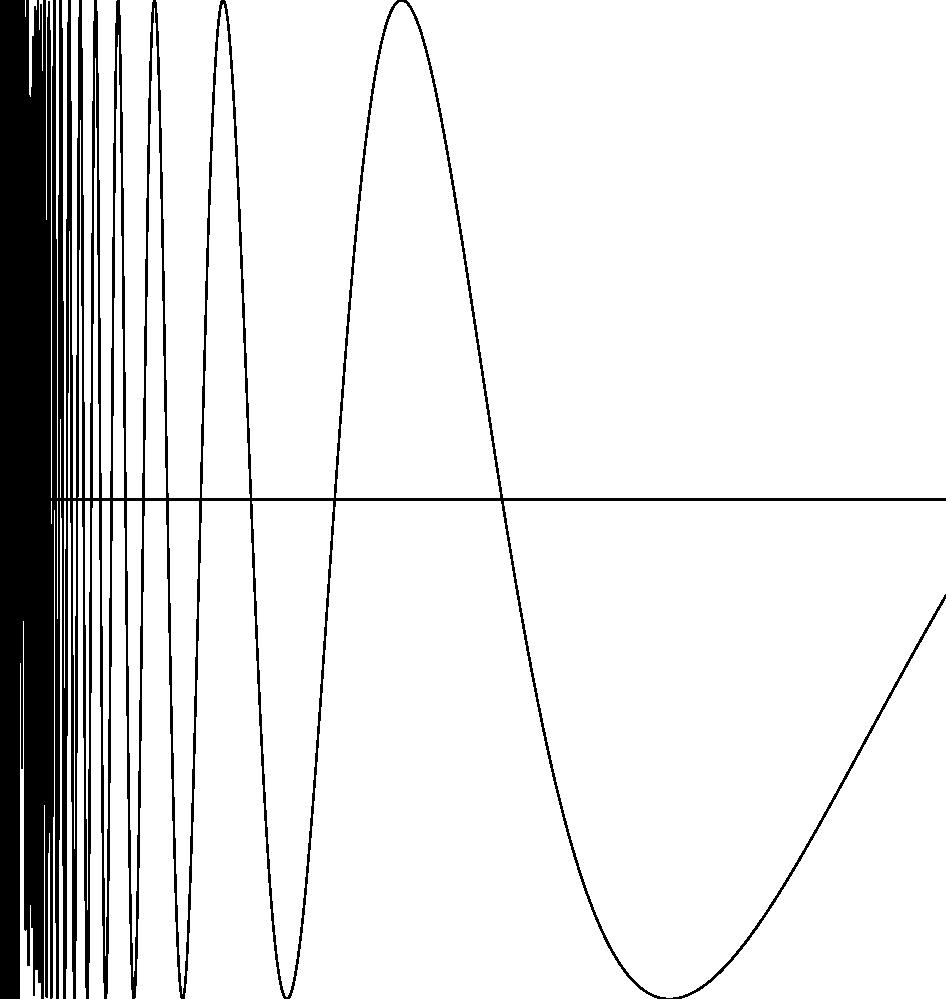
\includegraphics[width=0.4\linewidth]{sin_1_over_x.pdf}
    \end{center}
\end{example}
\begin{example}
    $y = \sqrt{x} \sin 1/x$, $y(0) = 0$, ее сумма оценивается $L \ge \sum_{n=1}^\infty \sqrt{\frac{1}{n}} = \infty$.
\end{example}
\begin{theorem}
    \[L = \int_a^b |\vf'(t)| dt \]
\end{theorem}
\begin{remark}
    $|\sum \vf_i| \le \sum |\vf_i|$, $||\vf| - |\vg|| \le |\vf - \vg|$, $|\int \vf dt| \le \int |\vf| dt$.
\end{remark}
\begin{longProof}
    Хотим доказать:
    \[\left| \int_a^b |\vf'(t)| dt - \sum_{i=1}^n |\vf(t_i) - \vf(t_{i-1})|\right| \to 0\]
    оценим это:
    \begin{multline*}
        \left| \int_a^b |\vf'(t)| dt - \sum_{i=1}^n |\vf(t_i) - \vf(t_{i-1})|\right| = \\
        \left| \int_a^b |\vf'(t)| dt - \sum_{i=1}^n |\vf'(\sigma_i)| \Delta_i t  + \sum_{i=1}^n |\vf' (\sigma_i)| \Delta_i t - \sum_{i=1}^n |\vf(t_i) - \vf(t_{i-1})| \right| \\
        \le \left| \int_a^b |\vf'(t)| dt - \sum_{i=1}^n |\vf'(\sigma_i)| \Delta_i t \right|  +\\
        \left| \sum_{i=1}^n |\vf' (\sigma_i)| \Delta_i t - \sum_{i=1}^n |\vf(t_i) - \vf(t_{i-1})| \right|
    \end{multline*}
    $\left| \int_a^b |\vf'(t)| dt - \sum_{i=1}^n |\vf'(\sigma_i)| \Delta_i t \right| \to 0$ по определению интеграла.

    $\vf'$ непрерывная, значит равномерно непрерывна, тогда если
    $\forall \epsilon > 0\  \exists \delta > 0\  |x_1 - x_2| < \delta \implies |\vf'(x_1) - \vf'(x_2)| < \epsilon$.
    Выберем любое $\epsilon$ и зафиксируем $\delta$, удовлетворяющее мелкости разбиения и получим:
    \begin{multline*}
        \left| \sum_{i=1}^n |\vf' (\sigma_i)| \Delta_i t - \sum_{i=1}^n |\vf(t_i) - \vf(t_{i-1})| \right| =\\
        \left|\sum_{i=1}^n \int_{t_{i-1}}^{t_i} |\vf'(\sigma_i)|dt -  \sum_{i=1}^n \left|\int_{t_{i-1}}^{t_i} \vf'(t)dt\right|\right|
        \le \sum_{i=1}^n \int_{t_{i-1}}^{t_i} \left|\vf'(\sigma_i) - \vf'(t) \right|dt \\
        \le \sum_{i=1}^n \int_{t_{i-1}}^{t_i} \epsilon dt = \epsilon (b-a) \to 0
    \end{multline*}
\end{longProof}

Попытаемся понять как вычислять длину прямой в некоторых случаях:\marginpar{12.09.22}
\begin{itemize}
    \item в случае явного задания:
          \begin{gather*}
              \displaystyle \begin{cases}
                  x = t \\
                  y = f(t)
              \end{cases} \Leftrightarrow y = f(t) \\
              |(x',y')|  = \sqrt{1 + \vf'^2(t)} \implies
              L = \int_a^b\sqrt{1 + \vf'^2(t)} dt
          \end{gather*}
          К сожалению, такая формула мало применима, так как интегралы берутся редко.
    \item в случае параметрического задания:
          \begin{gather*}\begin{cases}
                  x = x(t) \\
                  y = y(t) \\
                  z = z(t)
              \end{cases} \implies
              L = \int_a^b \sqrt{x'^2 + y'^2 +z'^2} dt
          \end{gather*}
    \item в случае полярных координат:
          \begin{gather*}
              r = r(\phi) \Leftrightarrow \begin{cases}
                  x = r(\phi) \cos \phi \\
                  y = r(\phi) \sin \phi
              \end{cases} \implies
              \begin{cases}
                  x' = r' \cos \phi -r \sin \phi \\
                  y' = r' \sin \phi + r \cos \phi
              \end{cases} \\
              \begin{multlined}
                  x'^2 + y'^2 = (r' \cos \phi -r \sin \phi)^2 + (r' \sin \phi + r \cos \phi)^2 = \\
                  r'^2\cos^2 \phi - 2rr'\sin \phi \cos \phi + r^2 \sin^2 \phi +\\
                  r'^2 \sin^2\phi + 2rr' \sin \phi \cos \phi + r^2 \cos^2 \phi = \\
                  r'^2 + r^2
              \end{multlined}\\
              L = \int_a^b \sqrt{x'^2 + y'^2} d\phi  = \int_a^b \sqrt{r'^2 + r^2}d \phi
          \end{gather*}
\end{itemize}
\end{document}